% $Id: appendix-a. $
% !TEX root = main.tex

\chapter{Appendixes}
\label{sec:appendixe}

\section{Evaluation Guide}
\label{sec:eval-guide}

\subsection{Introduction}
\subsubsection{Overview}
The objective of this research is to build a tool that allows the visualization of the behavior of a reinforcement 
learning agent and facilitates its debugging. Additionally, it is intended to understand the behavior of the RL 
agent during the training process, to help developers identify the main challenges in the correct operation of 
RL programs. The research has been carried out since January 2024 and will end in December 2024.
In this sense, Flik is a tool that will help your experience debugging a Reinforcement Learning program better. 
It is a python-based debugger and is done to be used only using the console. It will allow you to run your 
program step by step, check its variables and modify them during execution, and travel through time over 
the program.

\subsubsection{Requirements}
To be able to do this test you'll need to have docker installed or have a \href{https://labs.play-with-docker.com/}{play with docker} 
account. You will have to download a docker image, in which you will find all the useful tools installed in order to 
use Flik for three case scenarios for this test. Now, please follow the instructions for loading it in your computer 
in the following section.

\subsection{Installation}

\subsubsection{Option 1: Pull docker container (Recomended)}

Use the following command to download the docker image. And start running it on your computer or run it 
in \href{https://labs.play-with-docker.com/}{play with docker} page. To be able to run it in 
\href{https://labs.play-with-docker.com/}{play with docker}, create a new account and add a new instance 
(this might take a while, but is for free and on the web, so you don’t need to install docker).

\begin{lstlisting}[language=bash]
docker pull lrodriguez22/py-flik-debugger:latest
\end{lstlisting}

You can now run the following command:

\begin{lstlisting}[language=bash]
docker run -it lrodriguez22/py-flik-debugger
\end{lstlisting}

\subsubsection{Option 2: Download tar}
In case pulling the docker image is not working, you could download the docker container from this 
\href{docker container}{https://drive.google.com/file/d/1UpcZ6NZTvE9L12fV4NqpkAalY\_1x0xsS/view?usp=sharing}. 
Once you have downloaded the following .zip. Open a terminal and make sure you go to the path you download 
the .zip, then type:

\begin{lstlisting}[language=bash]
docker load -i py-flik-debugger.tar
\end{lstlisting}

This should take some minutes to complete. Once it has finished downloading, run the 
\href{docker container}{https://drive.google.com/file/d/1UpcZ6NZTvE9L12fV4NqpkAalY\_1x0xsS/view?usp=sharing} 
with the following command:

\begin{lstlisting}[language=bash]
docker run -it py-flik-debugger
\end{lstlisting}

\subsection{Getting Started}
\subsubsection{Launching Flik}

Once you are inside the container to use Flik just go use the following command:

\begin{lstlisting}[language=bash]
flik path_to_file/file.py
\end{lstlisting}

This will basically launch the debugger for the file you want to debug. Once you’ve done this, you should 
see an interface similar to the following image:

\begin{figure}[h]
    \centering
    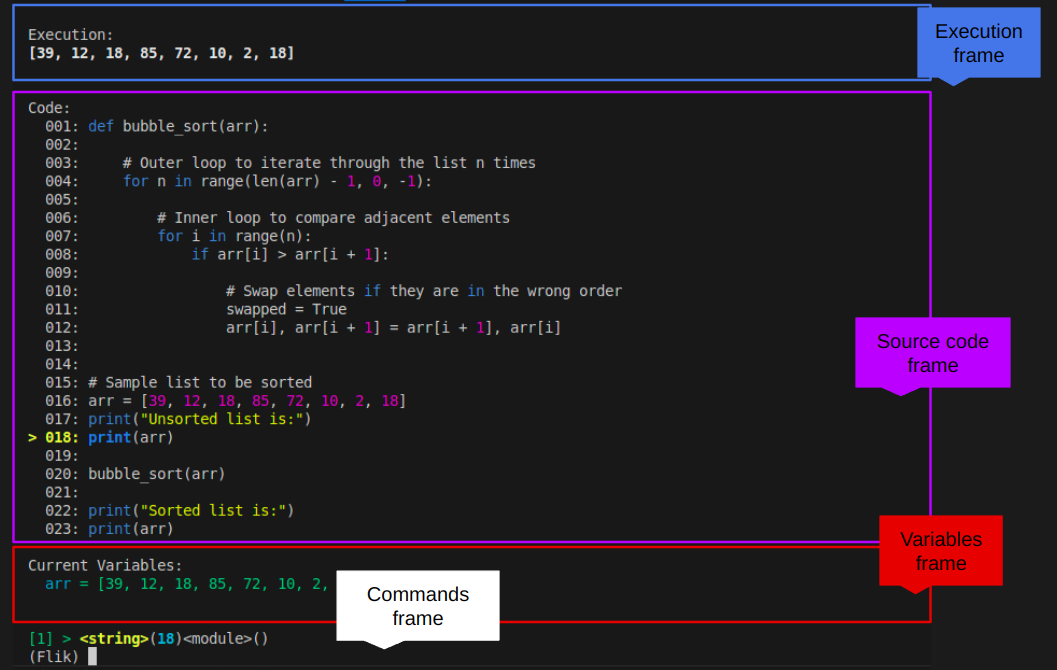
\includegraphics[width=1\textwidth]{figures/flik_interface.png}
    \caption{Debugger tool}
    \label{fig:debugger}
\end{figure}

Here, you should be able to see the current variables, the source code of the program you are running, 
and a console in which you will be able to interact with the code.

\subsubsection{Commands}
As almost all debuggers Flik lets you navigate through the code, the following list of commands will help 
you get started with Flik.

% Please add the following required packages to your document preamble:
% \usepackage[table,xcdraw]{xcolor}
% Beamer presentation requires \usepackage{colortbl} instead of \usepackage[table,xcdraw]{xcolor}
% \usepackage{longtable}
% Note: It may be necessary to compile the document several times to get a multi-page table to line up properly
\begin{longtable}[c]{cllll}
{\color[HTML]{222222} \textbf{Command}} & \multicolumn{1}{c}{{\color[HTML]{222222} \textbf{Description}}}                                                                                                                                                                                        & \multicolumn{1}{c}{} & \multicolumn{1}{c}{} & \multicolumn{1}{c}{} \\
\endfirsthead
%
\endhead
%
{\color[HTML]{222222} p}                & Print the value of an expression.                                                                                                                                                                                                                      &                      &                      &                      \\
{\color[HTML]{222222} pp}               & Pretty-print the value of an expression.                                                                                                                                                                                                               &                      &                      &                      \\
{\color[HTML]{222222} n}                & Continue execution until the next line in the current function is reached or it returns.                                                                                                                                                               &                      &                      &                      \\
{\color[HTML]{222222} s}                & \begin{tabular}[c]{@{}l@{}}Execute the current line and stop at the first possible occasion (either in a function \\ that is called or in the current function).\end{tabular}                                                                          &                      &                      &                      \\
{\color[HTML]{222222} c}                & Continue execution and only stop when a breakpoint is encountered.                                                                                                                                                                                     &                      &                      &                      \\
{\color[HTML]{222222} step\_back}       & goes one step in time from the line you are                                                                                                                                                                                                            &                      &                      &                      \\
{\color[HTML]{222222} back\_to}         & goes to the line you wish                                                                                                                                                                                                                              &                      &                      &                      \\
{\color[HTML]{222222} variables}        & shows the local and global variables from the current execution                                                                                                                                                                                        &                      &                      &                      \\
{\color[HTML]{222222} sticky}           & if you lose the pretty format of Flik you can go back by typing using this command.                                                                                                                                                                    &                      &                      &                      \\
{\color[HTML]{222222} args}             & To see the values of the function running right now.                                                                                                                                                                                                   &                      &                      &                      \\
{\color[HTML]{222222} setvar}           & \begin{tabular}[c]{@{}l@{}}It is a way in which you can modify a variable. Note that because of optimizations \\ of python, and variables protection this will not work in some cases.\end{tabular}                                                    &                      &                      &                      \\
{\color[HTML]{222222} unt}              & \begin{tabular}[c]{@{}l@{}}Continue execution until the line with a number greater than the current one is reached. \\ With a line number argument, continue execution until a line with a number greater or \\ equal to that is reached.\end{tabular} &                      &                      &                      \\
{\color[HTML]{222222} b}                & \begin{tabular}[c]{@{}l@{}}With no arguments, list all breaks. With a line number argument, set a breakpoint at \\ this line in the current file.\end{tabular}                                                                                         &                      &                      &                      \\
{\color[HTML]{222222} w}                & \begin{tabular}[c]{@{}l@{}}Print a stack trace, with the most recent frame at the bottom. An arrow indicates the \\ current frame, which determines the context of most commands.\end{tabular}                                                         &                      &                      &                      \\
{\color[HTML]{222222} u}                & Move the current frame count (default one) levels up in the stack trace (to an older frame).                                                                                                                                                           &                      &                      &                      \\
{\color[HTML]{222222} d}                & \begin{tabular}[c]{@{}l@{}}Move the current frame count (default one) levels down in the stack trace (to a newer \\ frame).\end{tabular}                                                                                                               &                      &                      &                      \\
{\color[HTML]{222222} help}             & See a list of available commands.                                                                                                                                                                                                                      &                      &                      &                      \\
{\color[HTML]{222222} q}                & Quit the debugger and exit.                                                                                                                                                                                                                            &                      &                      &                     
\label{tab:commands}
\end{longtable}

\subsection{Tasks Description}

The idea for every task is for you to find as many bugs as you can using Flik in each of the RL programs. 
For each task it is expected that you find the main bug hidden in the code. You are supposed to complete 
the following \href{https://forms.office.com/r/fg2AnRPfD1}{form} with that information. Good Luck!
In \href{https://github.com/larodriguez22/Flik_Experiments}{this link} you will find the experiments to be 
run for these tasks. Feel free to take a look and download them.

\subsubsection{Task 0: Example} 
In this task I will show you how to identify a bug using Flik. This is a basic example with an idea on what 
you are supposed to do. In this example we are using the division algorithm to divide two numbers. But 
we are missing something, we are not handling all the possible errors. If we run the following code it 
will work.

\begin{lstlisting}[language=Python]
def long_division(dividend, divisor):
    quotient = 0
    remainder = abs(dividend) 
    divisor = abs(divisor) 
    while remainder >= divisor:
        remainder -= divisor
        quotient += 1
    if (dividend < 0) != (divisor < 0): 
        quotient = -quotient
    return quotient, remainder

if __name__ == "__main__":
    dividend = 17
    divisor = 5
    quotient, remainder = long_division(dividend, divisor)
    print(f"Quotient: {quotient}")
    print(f"Remainder: {remainder}")
\end{lstlisting}

As you can see from the code above, there has been no code to handle division by zero, so if by mistake 
anyone would use the code placing divisor equal to zero, the code will get stuck in a loop. We can use Flik 
to run different examples of this code, to change the variables and to see why an error is happening, for 
example, we can go to line 23, which is going to have an error. Then we can run $s$, to get into the 
method. And see in real time the execution of the variables. At some point in the execution, we realized 
that for this case it is not working properly with our method. We then use the commands $back\_to$ 18. 
Then we change the variable divisor value to 2, and we go step by step again.

\begin{figure}[H]
    \centering
    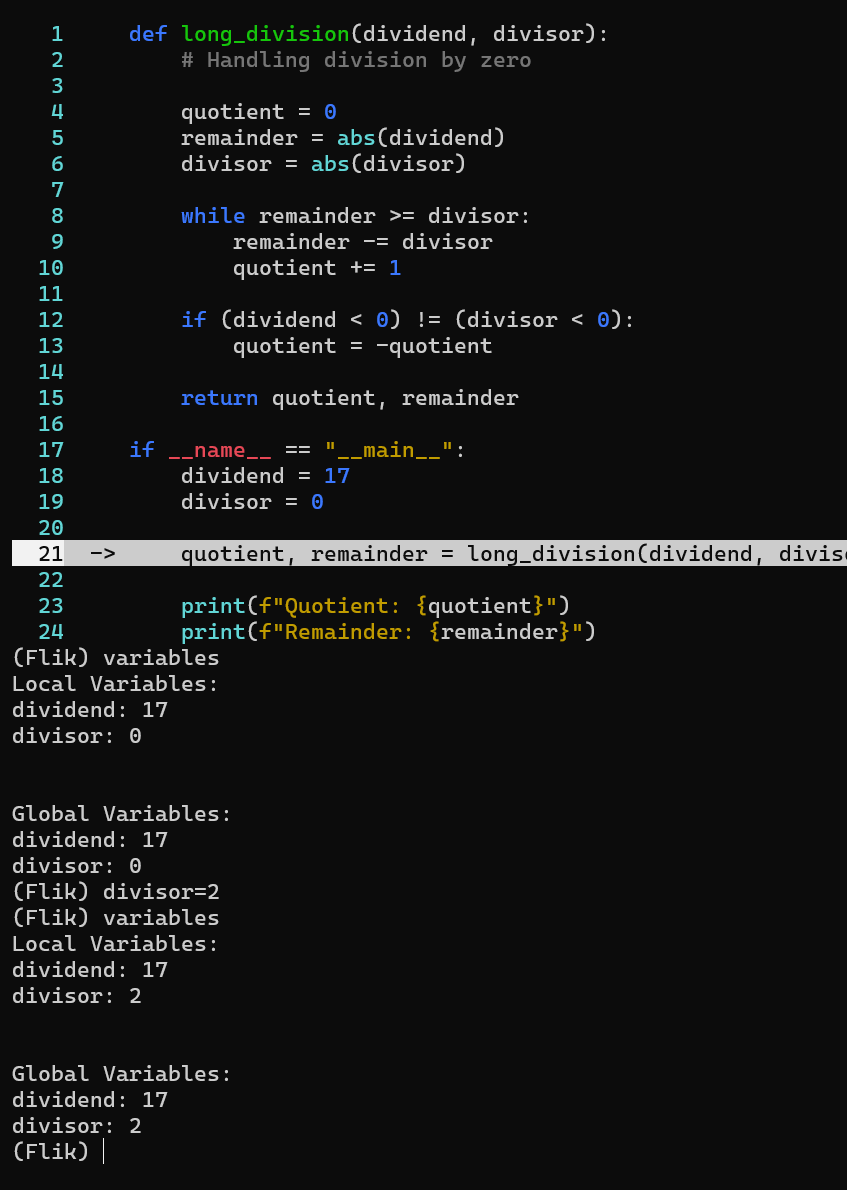
\includegraphics[width=0.3\textwidth]{figures/code_changes.png}
    \caption{Code example}
    \label{fig:code-example}
\end{figure}

Once we have realized the error, we can change the code and add the following exception:

\begin{lstlisting}[language=Python]
# Handling division by zero
if divisor == 0:
    raise ZeroDivisionError("Cannot divide by zero")
\end{lstlisting}

Now, it is your turn to find the bugs in these other tasks.

\subsubsection{Task 1: Gridworld}

The idea of this task is for you to figure out what is happening and what is the wrong behavior happening 
on this Reinforcement Learning program. The idea is for you to identify bugs on it. The gridworld 
environment consists of a $n\times n$ ($10\times 10$ in our example) rectangular board/grid, in which each tile $(i,j)$ 
represents a specific state of the board. Tiles in the board may be walls, which agents cannot cross. 
Additionally, there are special exit tiles that give a positive or negative reward to agents, as shown in 
\fref{fig:gridworld-code-example}. All tile types are unknown to the agent that moves from a given starting point in 
the board, searching for the goal state (\ie exit states with positive reward of $1$). The agent 
moves from state to state, avoiding obstacles and incorrect exit states (which give a reward of $-1$ 
when used to exit). For $25$ episodes, the result should look like:

\begin{figure}[H]
    \centering
    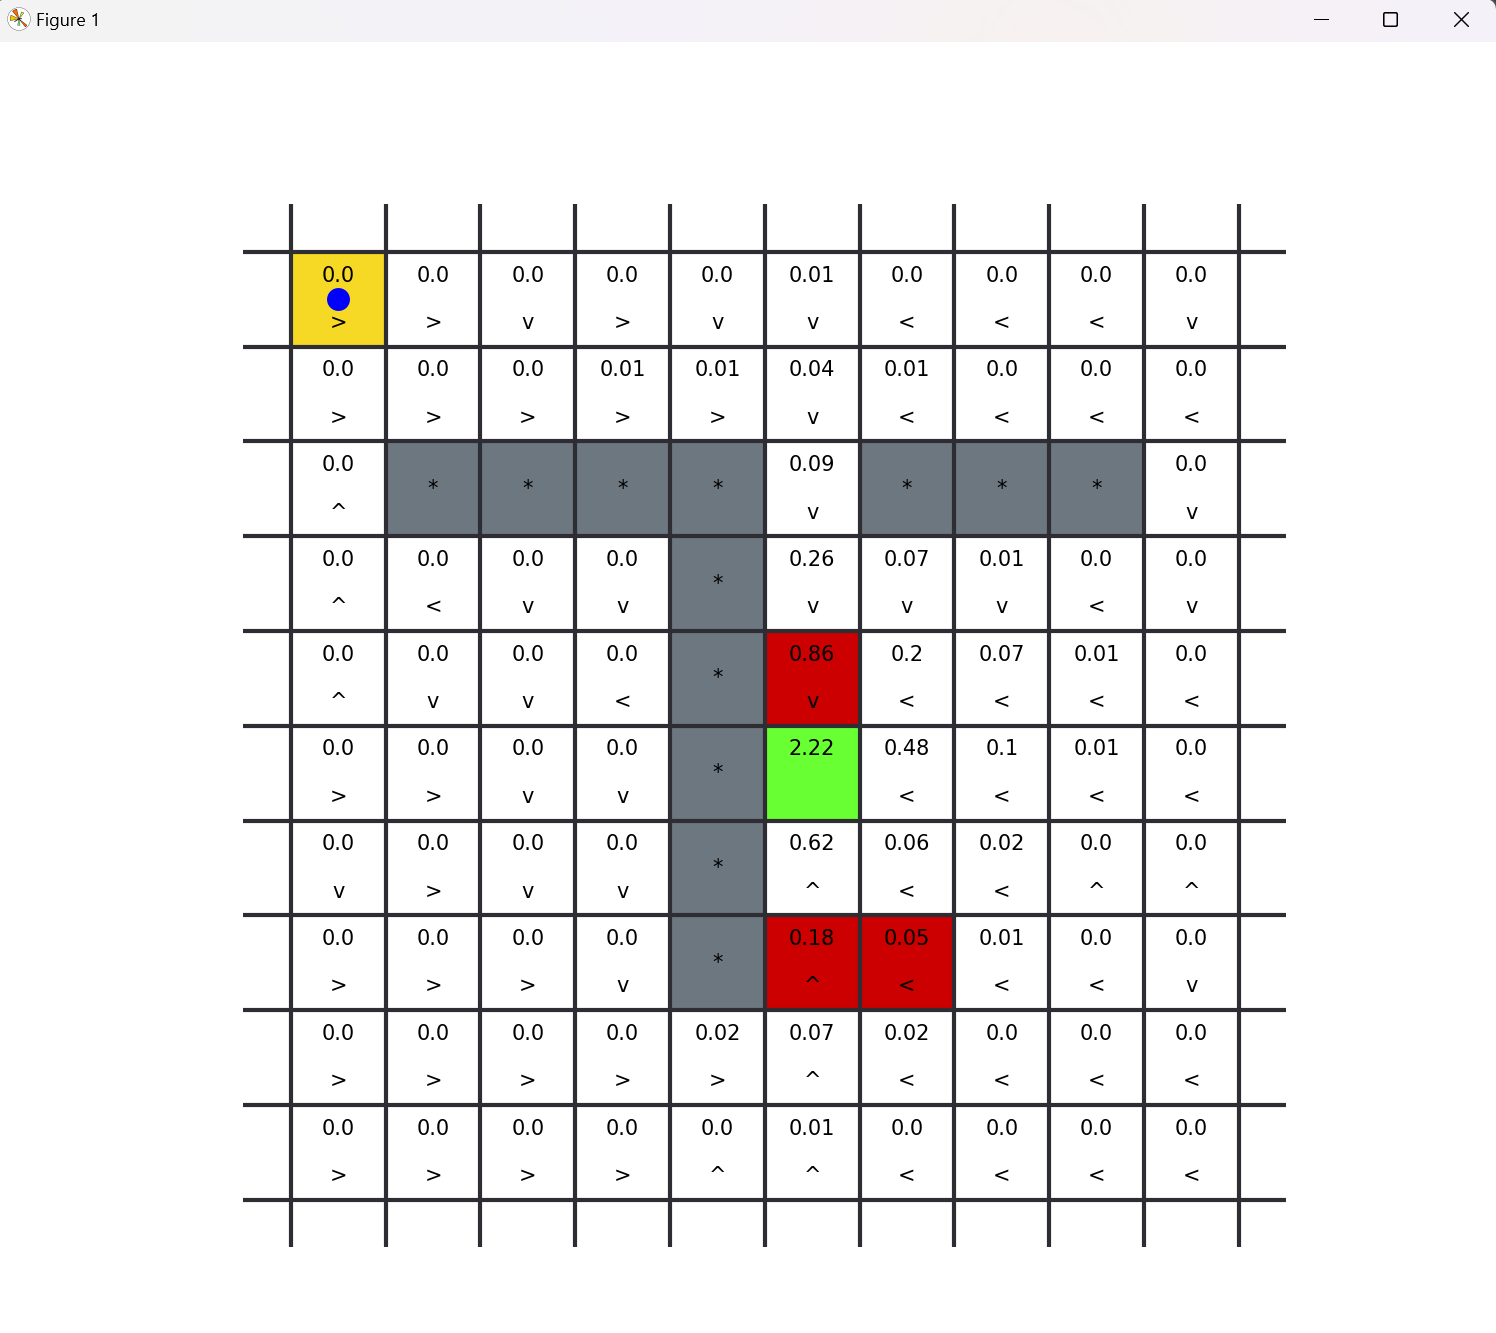
\includegraphics[width=0.5\textwidth]{figures/gridworld_example.png}
    \caption{Gridworld code example}
    \label{fig:gridworld-code-example}
\end{figure}

Note that the agent is learning so the values are being propagated on the Q-table. You can also run 
the gridworld experiment using the following command:

\begin{lstlisting}[language=bash]
python3 .\gridworld\gridworld.py
\end{lstlisting}

Also to run this using flik run (inside the docker container):

\begin{lstlisting}[language=bash]
flik experiments/gridworld/gridworld.py
\end{lstlisting}

\subsubsection{Task 2: Rooms}

The four rooms maze environment consists of a $13\times 13$ board/grid divided in $4$ sections, with walls 
between them, and a door opening to go from one room to another, as shown in \fref{fig:rooms}. 
The agent's objective in this environment is to exit through the upper-left room (the green square) 
in the fewest possible steps. Reaching the exit state gives a reward of $1$, and no other action gives a 
reward to the agent. In each episode the agent starts from any valid position in the grid, for example, 
the yellow square in the bottom-right room in the figure. For $25$ episodes, the results should look like:

\begin{figure}[H]
    \centering
    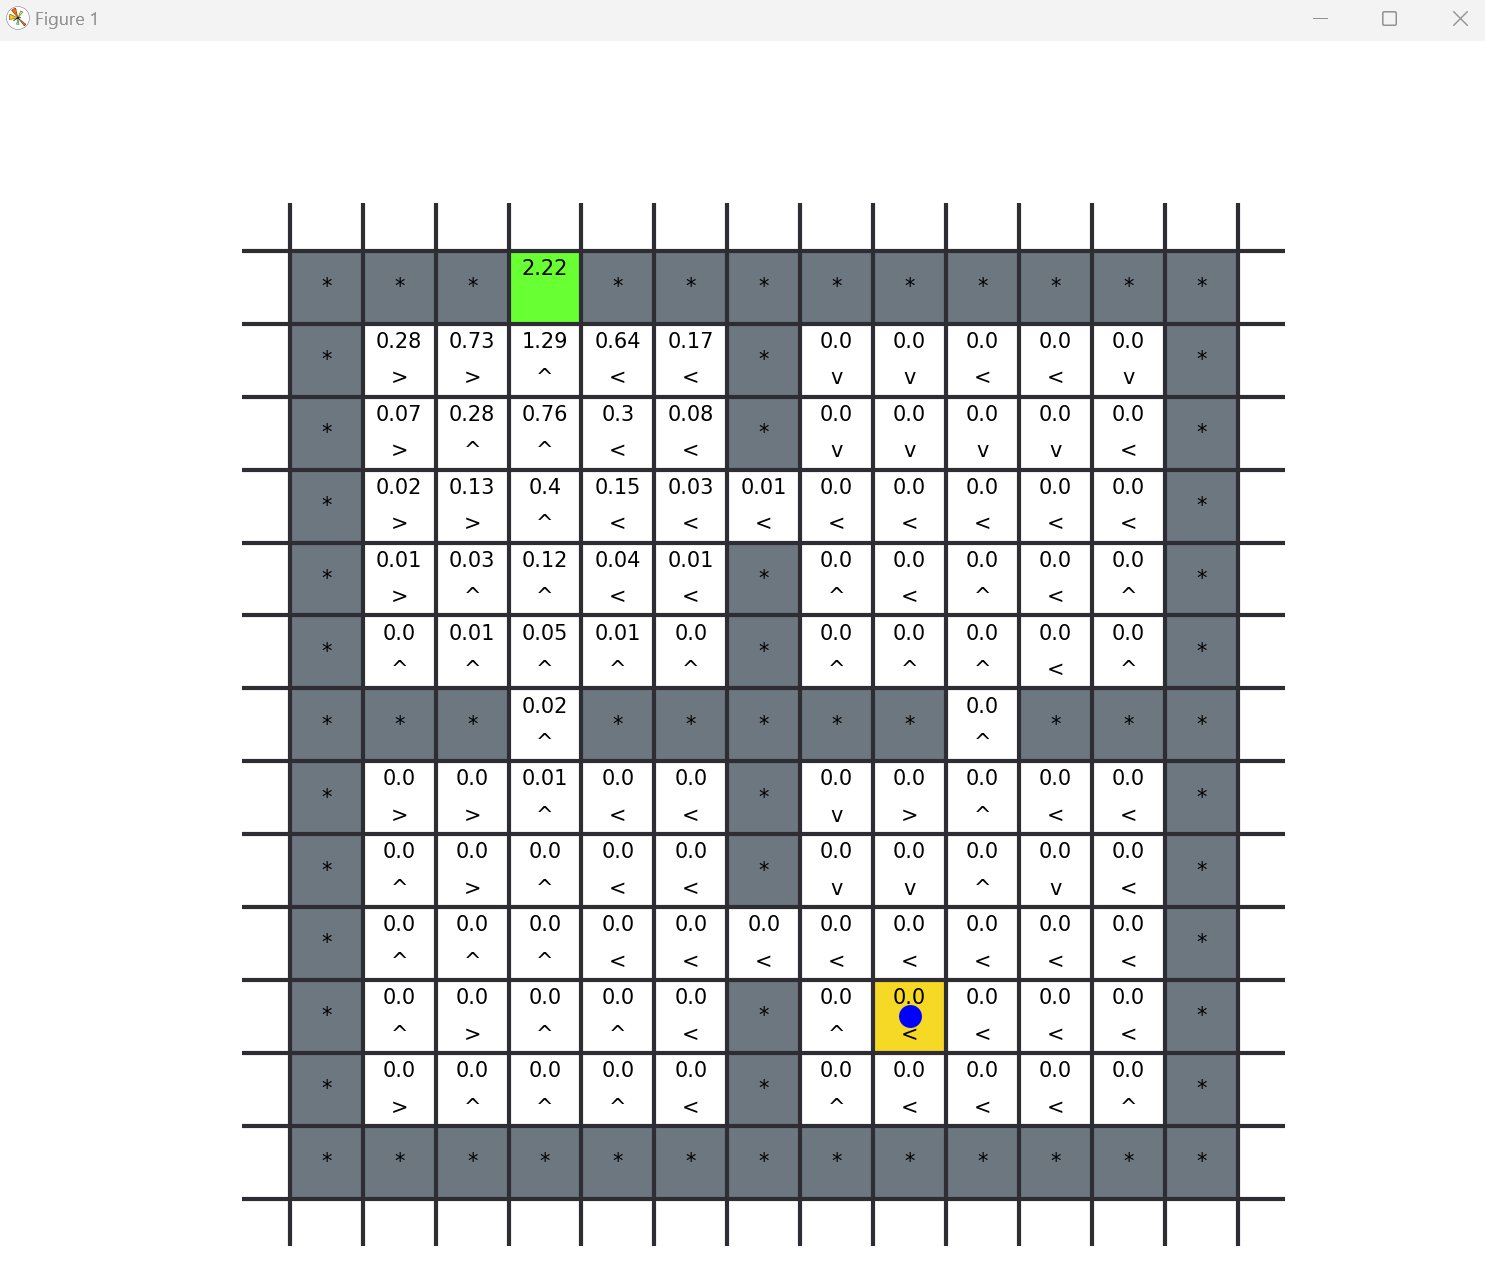
\includegraphics[width=0.5\textwidth]{figures/rooms_example.png}
    \caption{Rooms code example}
    \label{fig:rooms-code-example}
\end{figure}

Note the influence of the learning rate. You can also run the rooms experiment using the following command:

\begin{lstlisting}[language=bash]
python3 .\rooms\rooms.py
\end{lstlisting}

Also to run this using flik run (inside the docker container):

\begin{lstlisting}[language=bash]
flik experiments/rooms/rooms.py
\end{lstlisting}

\subsubsection{Task 3: Cars Example}

In this example the agent is basically learning how to drive. The idea of this task is that the agent 
goes as fast as possible on the road. In the road there are only two lanes, and there are other cars 
that the agent must pass without crashing on them. The possible actions for the agent are: straight, 
slow\_down, speed\_up, steer\_left, steer\_right. The following is the visual interface of this environment.

\begin{figure}[H]
    \centering
    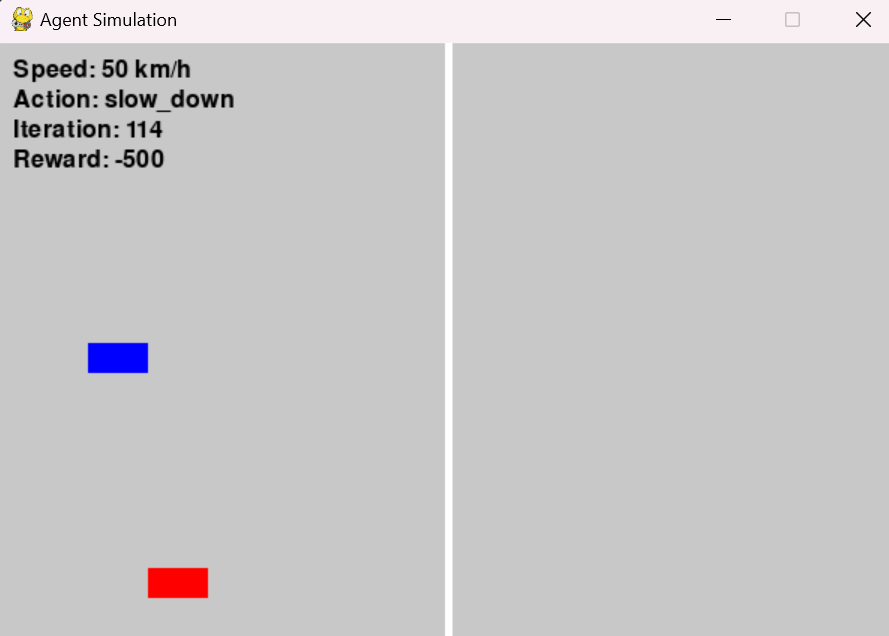
\includegraphics[width=0.5\textwidth]{figures/cars_example.png}
    \caption{Cars code example}
    \label{fig:cars-code-example}
\end{figure}

Note that we want the agent to learn how to drive at the maximum velocity allowed, we don’t want 
the agent to stop, or to crash. You can also run the rooms experiment using the following command:

\begin{lstlisting}[language=bash]
python3 .\cars\environment.py
\end{lstlisting}

Also to run this using flik run (inside the docker container):

\begin{lstlisting}[language=bash]
flik experiments/cars_example/environment.py
\end{lstlisting}

\section{Results}
\label{sec:appendix-results}

\subsection{General Knowledge Results}
\begin{figure}[H]
    \centering
    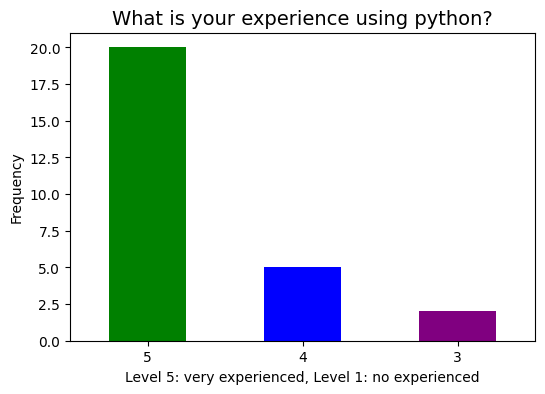
\includegraphics[width=0.5\textwidth]{figures/experience-python.png}
    \caption{Experience with Python}
    \label{fig:exp-py}
\end{figure}

\begin{figure}[H]
    \centering
    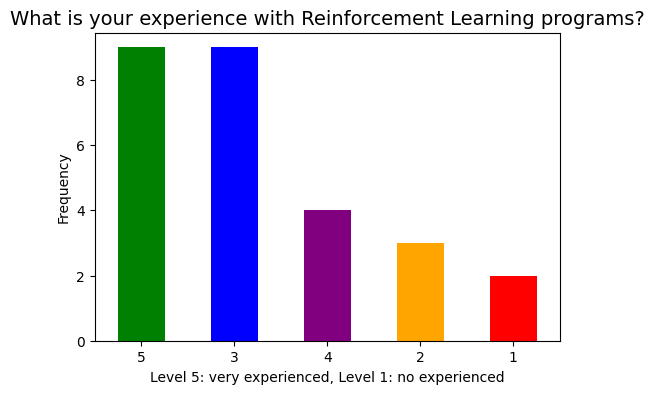
\includegraphics[width=0.5\textwidth]{figures/experience-rl.png}
    \caption{Experience with RL}
    \label{fig:exp-rl}
\end{figure}

\begin{figure}[H]
    \centering
    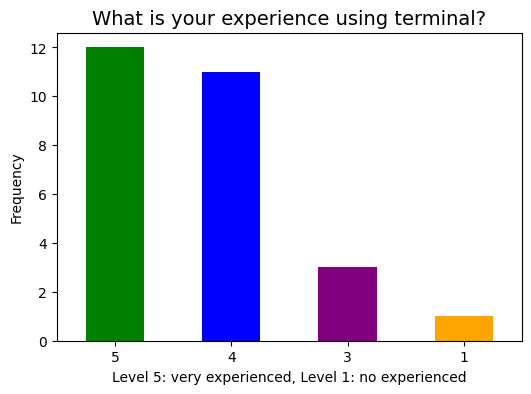
\includegraphics[width=0.5\textwidth]{figures/experience-terminal.png}
    \caption{Experience with Terminal}
    \label{fig:exp-terminal}
\end{figure}

\begin{figure}[H]
    \centering
    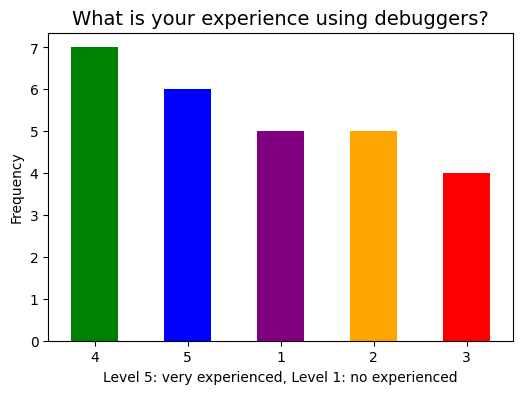
\includegraphics[width=0.5\textwidth]{figures/experience-debuggers.png}
    \caption{Experience with Debuggers}
    \label{fig:exp-deb}
\end{figure}


\subsection{Tasks Results}

\subsubsection{Task 1: Gridworld}

\begin{table}[H]
\centering
\resizebox{\columnwidth}{!}{%
\begin{tabular}{cccc}
\multicolumn{4}{c}{{\color[HTML]{000000} \textbf{Task 1: Gridworld Experiment.}}}                                                                                                                                                              \\
{\color[HTML]{000000} \textbf{Values}} & {\color[HTML]{000000} \textbf{Did you manage to finish the task?}} & {\color[HTML]{000000} \textbf{It was easy to solve the task}} & {\color[HTML]{000000} \textbf{Time it took you to find the bug}} \\
{\color[HTML]{000000} \textbf{5}}      & {\color[HTML]{000000} 15}                                        & {\color[HTML]{000000} 2}                                      & {\color[HTML]{000000} 2}                                         \\
{\color[HTML]{000000} \textbf{4}}      & {\color[HTML]{000000} 10}                                        & {\color[HTML]{000000} 16}                                     & {\color[HTML]{000000} 12}                                        \\
{\color[HTML]{000000} \textbf{3}}      & {\color[HTML]{000000} 2}                                         & {\color[HTML]{000000} 5}                                      & {\color[HTML]{000000} 4}                                         \\
{\color[HTML]{000000} \textbf{2}}      & {\color[HTML]{000000} 0}                                         & {\color[HTML]{000000} 3}                                      & {\color[HTML]{000000} 8}                                         \\
{\color[HTML]{000000} \textbf{1}}      & {\color[HTML]{000000} 0}                                         & {\color[HTML]{000000} 1}                                      & {\color[HTML]{000000} 1}                                        
\end{tabular}%
}
\caption{Gridworld Results}
\label{tab:grid-results}
\end{table}

\begin{figure}[H]
    \centering
    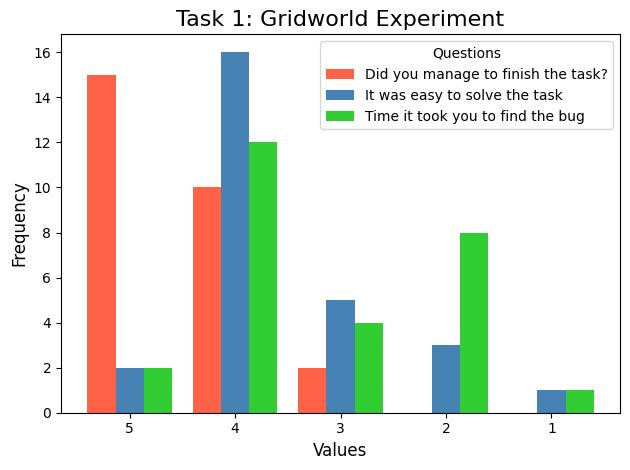
\includegraphics[width=0.5\textwidth]{figures/task1.png}
    \caption{Results Task 1}
    \label{fig:task1}
\end{figure}


\subsubsection{Task 2: Rooms}

\begin{table}[H]
\centering
\resizebox{\columnwidth}{!}{%
\begin{tabular}{
>{\columncolor[HTML]{FFFFFF}}c 
>{\columncolor[HTML]{FFFFFF}}c 
>{\columncolor[HTML]{FFFFFF}}c 
>{\columncolor[HTML]{FFFFFF}}c }
\multicolumn{4}{c}{\cellcolor[HTML]{FFFFFF}{\color[HTML]{000000} \textbf{Task 2: Rooms Experiment.}}}                                                                                                                                          \\
{\color[HTML]{000000} \textbf{Values}} & {\color[HTML]{000000} \textbf{Did you manage to finish the task?}} & {\color[HTML]{000000} \textbf{It was easy to solve the task}} & {\color[HTML]{000000} \textbf{Time it took you to find the bug}} \\
{\color[HTML]{000000} \textbf{4}}      & {\color[HTML]{000000} 13}                                          & {\color[HTML]{000000} 8}                                      & {\color[HTML]{000000} 5}                                         \\
{\color[HTML]{000000} \textbf{5}}      & {\color[HTML]{000000} 7}                                           & {\color[HTML]{000000} 1}                                      & {\color[HTML]{000000} 4}                                         \\
{\color[HTML]{000000} \textbf{3}}      & {\color[HTML]{000000} 4}                                           & {\color[HTML]{000000} 11}                                     & {\color[HTML]{000000} 9}                                         \\
{\color[HTML]{000000} \textbf{1}}      & {\color[HTML]{000000} 2}                                           & {\color[HTML]{000000} 1}                                      & {\color[HTML]{000000} 3}                                         \\
{\color[HTML]{000000} \textbf{2}}      & {\color[HTML]{000000} 1}                                           & {\color[HTML]{000000} 6}                                      & {\color[HTML]{000000} 6}                                        
\end{tabular}%
}
\caption{Rooms Results}
\label{tab:rooms-results}
\end{table}

\begin{figure}[H]
    \centering
    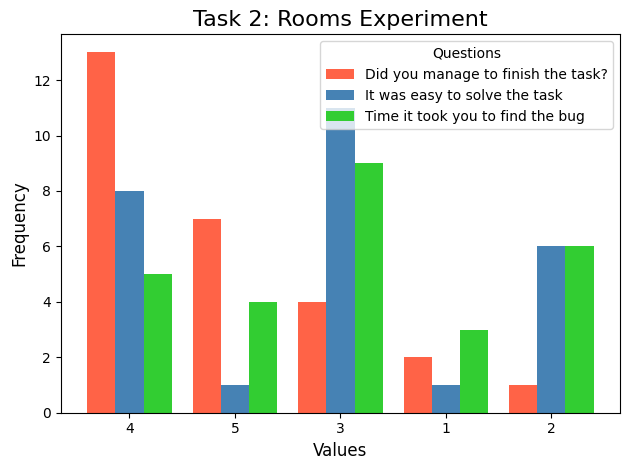
\includegraphics[width=0.5\textwidth]{figures/task2.png}
    \caption{Results Task 2}
    \label{fig:task2}
\end{figure}

\subsubsection{Task 3: Cars}

\begin{table}[H]
\centering
\resizebox{\columnwidth}{!}{%
\begin{tabular}{
>{\columncolor[HTML]{FFFFFF}}c 
>{\columncolor[HTML]{FFFFFF}}c 
>{\columncolor[HTML]{FFFFFF}}c 
>{\columncolor[HTML]{FFFFFF}}c }
\multicolumn{4}{c}{\cellcolor[HTML]{FFFFFF}{\color[HTML]{000000} \textbf{Task 3: Cars Experiment.}}}                                                                                                                                           \\
{\color[HTML]{000000} \textbf{Values}} & {\color[HTML]{000000} \textbf{Did you manage to finish the task?}} & {\color[HTML]{000000} \textbf{It was easy to solve the task}} & {\color[HTML]{000000} \textbf{Time it took you to find the bug}} \\
{\color[HTML]{000000} \textbf{5}}      & {\color[HTML]{000000} 8}                                           & {\color[HTML]{000000} 2}                                      & {\color[HTML]{000000} 6}                                         \\
{\color[HTML]{000000} \textbf{3}}      & {\color[HTML]{000000} 6}                                           & {\color[HTML]{000000} 7}                                      & {\color[HTML]{000000} 6}                                         \\
{\color[HTML]{000000} \textbf{4}}      & {\color[HTML]{000000} 6}                                           & {\color[HTML]{000000} 4}                                      & {\color[HTML]{000000} 5}                                         \\
{\color[HTML]{000000} \textbf{2}}      & {\color[HTML]{000000} 4}                                           & {\color[HTML]{000000} 10}                                     & {\color[HTML]{000000} 7}                                         \\
{\color[HTML]{000000} \textbf{1}}      & {\color[HTML]{000000} 3}                                           & {\color[HTML]{000000} 4}                                      & {\color[HTML]{000000} 3}                                        
\end{tabular}%
}
\caption{Cars Results}
\label{tab:cars-results}
\end{table}

\begin{figure}[H]
    \centering
    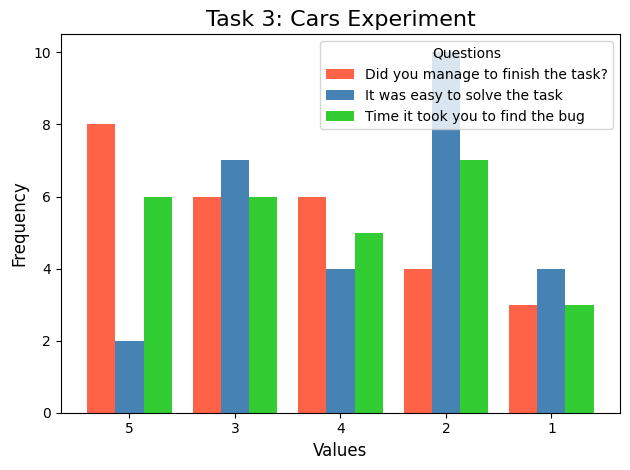
\includegraphics[width=0.5\textwidth]{figures/task3.png}
    \caption{Results Task 3}
    \label{fig:task3}
\end{figure}

\subsection{Debugger Usability}

% Tabla larga horizontal
\begin{landscape}
\begin{table}[]
\centering
\resizebox{\columnwidth}{!}{%
\begin{tabular}{
>{\columncolor[HTML]{FFFFFF}}c 
>{\columncolor[HTML]{FFFFFF}}c 
>{\columncolor[HTML]{FFFFFF}}c 
>{\columncolor[HTML]{FFFFFF}}c 
>{\columncolor[HTML]{FFFFFF}}c 
>{\columncolor[HTML]{FFFFFF}}c 
>{\columncolor[HTML]{FFFFFF}}c 
>{\columncolor[HTML]{FFFFFF}}c 
>{\columncolor[HTML]{FFFFFF}}c 
>{\columncolor[HTML]{FFFFFF}}c 
>{\columncolor[HTML]{FFFFFF}}c }
\multicolumn{11}{c}{\cellcolor[HTML]{FFFFFF}{\color[HTML]{383838} \textbf{Task 2: Rooms Experiment.}}}                                                                                                                                                                                                                                                                                                                                                                                                                                                                                                                                                                                                                                                                                                                                                                                                                                                                                                                                                                                                                                                                                                                                                                                                                                                         \\
{\color[HTML]{383838} \textbf{}}  & {\color[HTML]{383838} \textbf{\begin{tabular}[c]{@{}c@{}}I think I would like to use this \\ system frequently\end{tabular}}} & {\color[HTML]{383838} \textbf{\begin{tabular}[c]{@{}c@{}}I find this system \\ unnecessarily complex\end{tabular}}} & {\color[HTML]{383838} \textbf{\begin{tabular}[c]{@{}c@{}}I think the system \\ is easy to use\end{tabular}}} & {\color[HTML]{383838} \textbf{\begin{tabular}[c]{@{}c@{}}I think I would need technical \\ support to use the system\end{tabular}}} & {\color[HTML]{383838} \textbf{\begin{tabular}[c]{@{}c@{}}I find the various functions of the \\ system quite well integrated\end{tabular}}} & {\color[HTML]{383838} \textbf{\begin{tabular}[c]{@{}c@{}}I have found too much \\ inconsistency in this system\end{tabular}}} & {\color[HTML]{383838} \textbf{\begin{tabular}[c]{@{}c@{}}I think most people would learn \\ to use the system quickly\end{tabular}}} & {\color[HTML]{383838} \textbf{\begin{tabular}[c]{@{}c@{}}I found the system quite \\ awkward to use\end{tabular}}} & {\color[HTML]{383838} \textbf{\begin{tabular}[c]{@{}c@{}}I have felt very safe \\ using the system\end{tabular}}} & {\color[HTML]{383838} \textbf{\begin{tabular}[c]{@{}c@{}}I would need to learn a lot \\ of things before I could handle the system\end{tabular}}} \\
{\color[HTML]{383838} \textbf{5}} & {\color[HTML]{383838} 7}                                                                                                      & {\color[HTML]{383838} 2}                                                                                            & {\color[HTML]{383838} 5.0}                                                                                   & {\color[HTML]{383838} 9}                                                                                                            & {\color[HTML]{383838} 6}                                                                                                                    & {\color[HTML]{383838} 1}                                                                                                      & {\color[HTML]{383838} 7}                                                                                                             & {\color[HTML]{383838} 4}                                                                                           & {\color[HTML]{383838} 7}                                                                                          & {\color[HTML]{383838} 8.0}                                                                                                                        \\
{\color[HTML]{383838} \textbf{2}} & {\color[HTML]{383838} 7}                                                                                                      & {\color[HTML]{383838} 6}                                                                                            & {\color[HTML]{383838} 6.0}                                                                                   & {\color[HTML]{383838} 3}                                                                                                            & {\color[HTML]{383838} 2}                                                                                                                    & {\color[HTML]{383838} 7}                                                                                                      & {\color[HTML]{383838} 6}                                                                                                             & {\color[HTML]{383838} 4}                                                                                           & {\color[HTML]{383838} 4}                                                                                          & {\color[HTML]{383838} NaN}                                                                                                                        \\
{\color[HTML]{383838} \textbf{3}} & {\color[HTML]{383838} 7}                                                                                                      & {\color[HTML]{383838} 7}                                                                                            & {\color[HTML]{383838} 11.0}                                                                                  & {\color[HTML]{383838} 4}                                                                                                            & {\color[HTML]{383838} 5}                                                                                                                    & {\color[HTML]{383838} 4}                                                                                                      & {\color[HTML]{383838} 6}                                                                                                             & {\color[HTML]{383838} 9}                                                                                           & {\color[HTML]{383838} 7}                                                                                          & {\color[HTML]{383838} 4.0}                                                                                                                        \\
{\color[HTML]{383838} \textbf{4}} & {\color[HTML]{383838} 5}                                                                                                      & {\color[HTML]{383838} 7}                                                                                            & {\color[HTML]{383838} 5.0}                                                                                   & {\color[HTML]{383838} 8}                                                                                                            & {\color[HTML]{383838} 13}                                                                                                                   & {\color[HTML]{383838} 2}                                                                                                      & {\color[HTML]{383838} 6}                                                                                                             & {\color[HTML]{383838} 7}                                                                                           & {\color[HTML]{383838} 8}                                                                                          & {\color[HTML]{383838} 6.0}                                                                                                                        \\
{\color[HTML]{383838} \textbf{1}} & {\color[HTML]{383838} 1}                                                                                                      & {\color[HTML]{383838} 5}                                                                                            & {\color[HTML]{383838} NaN}                                                                                   & {\color[HTML]{383838} 3}                                                                                                            & {\color[HTML]{383838} 1}                                                                                                                    & {\color[HTML]{383838} 13}                                                                                                     & {\color[HTML]{383838} 2}                                                                                                             & {\color[HTML]{383838} 3}                                                                                           & {\color[HTML]{383838} 1}                                                                                          & {\color[HTML]{383838} 9.0}                                                                                                                       
\end{tabular}%
}
\end{table}
\end{landscape}

% % Tabla corta 1, horizontal
% \begin{landscape}
% \begin{table}[]
% \centering
% \resizebox{\columnwidth}{!}{%
% \begin{tabular}{
% >{\columncolor[HTML]{FFFFFF}}c 
% >{\columncolor[HTML]{FFFFFF}}c 
% >{\columncolor[HTML]{FFFFFF}}c 
% >{\columncolor[HTML]{FFFFFF}}c 
% >{\columncolor[HTML]{FFFFFF}}c 
% >{\columncolor[HTML]{FFFFFF}}c }
% \multicolumn{6}{c}{\cellcolor[HTML]{FFFFFF}{\color[HTML]{383838} \textbf{Task 2: Rooms Experiment.}}}                                                                                                                                                                                                                                                                                                                                                                                                                                                                                                                                                                                      \\
% {\color[HTML]{383838} \textbf{}}  & {\color[HTML]{383838} \textbf{\begin{tabular}[c]{@{}c@{}}I think I would like to use this \\ system frequently\end{tabular}}} & {\color[HTML]{383838} \textbf{\begin{tabular}[c]{@{}c@{}}I find this system \\ unnecessarily complex\end{tabular}}} & {\color[HTML]{383838} \textbf{\begin{tabular}[c]{@{}c@{}}I think the system \\ is easy to use\end{tabular}}} & {\color[HTML]{383838} \textbf{\begin{tabular}[c]{@{}c@{}}I think I would need technical \\ support to use the system\end{tabular}}} & {\color[HTML]{383838} \textbf{\begin{tabular}[c]{@{}c@{}}I find the various functions of the \\ system quite well integrated\end{tabular}}} \\
% {\color[HTML]{383838} \textbf{5}} & {\color[HTML]{383838} 7}                                                                                                      & {\color[HTML]{383838} 2}                                                                                            & {\color[HTML]{383838} 5.0}                                                                                   & {\color[HTML]{383838} 9}                                                                                                            & {\color[HTML]{383838} 6}                                                                                                                    \\
% {\color[HTML]{383838} \textbf{2}} & {\color[HTML]{383838} 7}                                                                                                      & {\color[HTML]{383838} 6}                                                                                            & {\color[HTML]{383838} 6.0}                                                                                   & {\color[HTML]{383838} 3}                                                                                                            & {\color[HTML]{383838} 2}                                                                                                                    \\
% {\color[HTML]{383838} \textbf{3}} & {\color[HTML]{383838} 7}                                                                                                      & {\color[HTML]{383838} 7}                                                                                            & {\color[HTML]{383838} 11.0}                                                                                  & {\color[HTML]{383838} 4}                                                                                                            & {\color[HTML]{383838} 5}                                                                                                                    \\
% {\color[HTML]{383838} \textbf{4}} & {\color[HTML]{383838} 5}                                                                                                      & {\color[HTML]{383838} 7}                                                                                            & {\color[HTML]{383838} 5.0}                                                                                   & {\color[HTML]{383838} 8}                                                                                                            & {\color[HTML]{383838} 13}                                                                                                                   \\
% {\color[HTML]{383838} \textbf{1}} & {\color[HTML]{383838} 1}                                                                                                      & {\color[HTML]{383838} 5}                                                                                            & {\color[HTML]{383838} NaN}                                                                                   & {\color[HTML]{383838} 3}                                                                                                            & {\color[HTML]{383838} 1}                                                                                                                   
% \end{tabular}%
% }
% \end{table}
% \end{landscape}


% % Tabla corta 2 horizontal
% \begin{landscape}
% \begin{table}[]
% \centering
% \resizebox{\columnwidth}{!}{%
% \begin{tabular}{
% >{\columncolor[HTML]{FFFFFF}}c 
% >{\columncolor[HTML]{FFFFFF}}c 
% >{\columncolor[HTML]{FFFFFF}}c 
% >{\columncolor[HTML]{FFFFFF}}c 
% >{\columncolor[HTML]{FFFFFF}}c 
% >{\columncolor[HTML]{FFFFFF}}c }
% \multicolumn{6}{c}{\cellcolor[HTML]{FFFFFF}{\color[HTML]{383838} \textbf{Task 2: Rooms Experiment.}}}                                                                                                                                                                                                                                                                                                                                                                                                                                                                                                                                                                                                 \\
% {\color[HTML]{383838} \textbf{}}  & {\color[HTML]{383838} \textbf{\begin{tabular}[c]{@{}c@{}}I have found too much \\ inconsistency in this system\end{tabular}}} & {\color[HTML]{383838} \textbf{\begin{tabular}[c]{@{}c@{}}I think most people would learn \\ to use the system quickly\end{tabular}}} & {\color[HTML]{383838} \textbf{\begin{tabular}[c]{@{}c@{}}I found the system quite \\ awkward to use\end{tabular}}} & {\color[HTML]{383838} \textbf{\begin{tabular}[c]{@{}c@{}}I have felt very safe \\ using the system\end{tabular}}} & {\color[HTML]{383838} \textbf{\begin{tabular}[c]{@{}c@{}}I would need to learn a lot \\ of things before I could handle the system\end{tabular}}} \\
% {\color[HTML]{383838} \textbf{5}} & {\color[HTML]{383838} 1}                                                                                                      & {\color[HTML]{383838} 7}                                                                                                             & {\color[HTML]{383838} 4}                                                                                           & {\color[HTML]{383838} 7}                                                                                          & {\color[HTML]{383838} 8.0}                                                                                                                        \\
% {\color[HTML]{383838} \textbf{2}} & {\color[HTML]{383838} 7}                                                                                                      & {\color[HTML]{383838} 6}                                                                                                             & {\color[HTML]{383838} 4}                                                                                           & {\color[HTML]{383838} 4}                                                                                          & {\color[HTML]{383838} NaN}                                                                                                                        \\
% {\color[HTML]{383838} \textbf{3}} & {\color[HTML]{383838} 4}                                                                                                      & {\color[HTML]{383838} 6}                                                                                                             & {\color[HTML]{383838} 9}                                                                                           & {\color[HTML]{383838} 7}                                                                                          & {\color[HTML]{383838} 4.0}                                                                                                                        \\
% {\color[HTML]{383838} \textbf{4}} & {\color[HTML]{383838} 2}                                                                                                      & {\color[HTML]{383838} 6}                                                                                                             & {\color[HTML]{383838} 7}                                                                                           & {\color[HTML]{383838} 8}                                                                                          & {\color[HTML]{383838} 6.0}                                                                                                                        \\
% {\color[HTML]{383838} \textbf{1}} & {\color[HTML]{383838} 13}                                                                                                     & {\color[HTML]{383838} 2}                                                                                                             & {\color[HTML]{383838} 3}                                                                                           & {\color[HTML]{383838} 1}                                                                                          & {\color[HTML]{383838} 9.0}                                                                                                                       
% \end{tabular}%
% }
% \end{table}
% \end{landscape}

% Tabla corta 1 
% \begin{table}[H]
% \centering
% \resizebox{\columnwidth}{!}{%
% \begin{tabular}{
% >{\columncolor[HTML]{FFFFFF}}c 
% >{\columncolor[HTML]{FFFFFF}}c 
% >{\columncolor[HTML]{FFFFFF}}c 
% >{\columncolor[HTML]{FFFFFF}}c 
% >{\columncolor[HTML]{FFFFFF}}c 
% >{\columncolor[HTML]{FFFFFF}}c }
% \multicolumn{6}{c}{\cellcolor[HTML]{FFFFFF}{\color[HTML]{383838} \textbf{Task 2: Rooms Experiment.}}}                                                                                                                                                                                                                                                                                                                                                                                                                                                                                                                                                                                                 \\
% {\color[HTML]{383838} \textbf{}}  & {\color[HTML]{383838} \textbf{\begin{tabular}[c]{@{}c@{}}I have found too much \\ inconsistency in this system\end{tabular}}} & {\color[HTML]{383838} \textbf{\begin{tabular}[c]{@{}c@{}}I think most people would learn \\ to use the system quickly\end{tabular}}} & {\color[HTML]{383838} \textbf{\begin{tabular}[c]{@{}c@{}}I found the system quite \\ awkward to use\end{tabular}}} & {\color[HTML]{383838} \textbf{\begin{tabular}[c]{@{}c@{}}I have felt very safe \\ using the system\end{tabular}}} & {\color[HTML]{383838} \textbf{\begin{tabular}[c]{@{}c@{}}I would need to learn a lot \\ of things before I could handle the system\end{tabular}}} \\
% {\color[HTML]{383838} \textbf{5}} & {\color[HTML]{383838} 1}                                                                                                      & {\color[HTML]{383838} 7}                                                                                                             & {\color[HTML]{383838} 4}                                                                                           & {\color[HTML]{383838} 7}                                                                                          & {\color[HTML]{383838} 8.0}                                                                                                                        \\
% {\color[HTML]{383838} \textbf{2}} & {\color[HTML]{383838} 7}                                                                                                      & {\color[HTML]{383838} 6}                                                                                                             & {\color[HTML]{383838} 4}                                                                                           & {\color[HTML]{383838} 4}                                                                                          & {\color[HTML]{383838} NaN}                                                                                                                        \\
% {\color[HTML]{383838} \textbf{3}} & {\color[HTML]{383838} 4}                                                                                                      & {\color[HTML]{383838} 6}                                                                                                             & {\color[HTML]{383838} 9}                                                                                           & {\color[HTML]{383838} 7}                                                                                          & {\color[HTML]{383838} 4.0}                                                                                                                        \\
% {\color[HTML]{383838} \textbf{4}} & {\color[HTML]{383838} 2}                                                                                                      & {\color[HTML]{383838} 6}                                                                                                             & {\color[HTML]{383838} 7}                                                                                           & {\color[HTML]{383838} 8}                                                                                          & {\color[HTML]{383838} 6.0}                                                                                                                        \\
% {\color[HTML]{383838} \textbf{1}} & {\color[HTML]{383838} 13}                                                                                                     & {\color[HTML]{383838} 2}                                                                                                             & {\color[HTML]{383838} 3}                                                                                           & {\color[HTML]{383838} 1}                                                                                          & {\color[HTML]{383838} 9.0}                                                                                                                       
% \end{tabular}%
% }
% \caption{General Results Part 1}
% \label{tab:general1-debuggers}
% \end{table}

% Tabla corta 2
% \begin{table}[H]
% \centering
% \resizebox{\columnwidth}{!}{%
% \begin{tabular}{
% >{\columncolor[HTML]{FFFFFF}}c 
% >{\columncolor[HTML]{FFFFFF}}c 
% >{\columncolor[HTML]{FFFFFF}}c 
% >{\columncolor[HTML]{FFFFFF}}c 
% >{\columncolor[HTML]{FFFFFF}}c 
% >{\columncolor[HTML]{FFFFFF}}c }
% \multicolumn{6}{c}{\cellcolor[HTML]{FFFFFF}{\color[HTML]{383838} \textbf{Task 2: Rooms Experiment.}}}                                                                                                                                                                                                                                                                                                                                                                                                                                                                                                                                                                                      \\
% {\color[HTML]{383838} \textbf{}}  & {\color[HTML]{383838} \textbf{\begin{tabular}[c]{@{}c@{}}I think I would like to use this \\ system frequently\end{tabular}}} & {\color[HTML]{383838} \textbf{\begin{tabular}[c]{@{}c@{}}I find this system \\ unnecessarily complex\end{tabular}}} & {\color[HTML]{383838} \textbf{\begin{tabular}[c]{@{}c@{}}I think the system \\ is easy to use\end{tabular}}} & {\color[HTML]{383838} \textbf{\begin{tabular}[c]{@{}c@{}}I think I would need technical \\ support to use the system\end{tabular}}} & {\color[HTML]{383838} \textbf{\begin{tabular}[c]{@{}c@{}}I find the various functions of the \\ system quite well integrated\end{tabular}}} \\
% {\color[HTML]{383838} \textbf{5}} & {\color[HTML]{383838} 7}                                                                                                      & {\color[HTML]{383838} 2}                                                                                            & {\color[HTML]{383838} 5.0}                                                                                   & {\color[HTML]{383838} 9}                                                                                                            & {\color[HTML]{383838} 6}                                                                                                                    \\
% {\color[HTML]{383838} \textbf{2}} & {\color[HTML]{383838} 7}                                                                                                      & {\color[HTML]{383838} 6}                                                                                            & {\color[HTML]{383838} 6.0}                                                                                   & {\color[HTML]{383838} 3}                                                                                                            & {\color[HTML]{383838} 2}                                                                                                                    \\
% {\color[HTML]{383838} \textbf{3}} & {\color[HTML]{383838} 7}                                                                                                      & {\color[HTML]{383838} 7}                                                                                            & {\color[HTML]{383838} 11.0}                                                                                  & {\color[HTML]{383838} 4}                                                                                                            & {\color[HTML]{383838} 5}                                                                                                                    \\
% {\color[HTML]{383838} \textbf{4}} & {\color[HTML]{383838} 5}                                                                                                      & {\color[HTML]{383838} 7}                                                                                            & {\color[HTML]{383838} 5.0}                                                                                   & {\color[HTML]{383838} 8}                                                                                                            & {\color[HTML]{383838} 13}                                                                                                                   \\
% {\color[HTML]{383838} \textbf{1}} & {\color[HTML]{383838} 1}                                                                                                      & {\color[HTML]{383838} 5}                                                                                            & {\color[HTML]{383838} NaN}                                                                                   & {\color[HTML]{383838} 3}                                                                                                            & {\color[HTML]{383838} 1}                                                                                                                   
% \end{tabular}%
% }
% \caption{General Results Part 2}
% \label{tab:general2-debuggers}
% \end{table}



\endinput

